\newcommand{\posterPolarimeters}[1]{

\setlength{\frameWidth}{#1}
\setlength{\unitlength}{0.02\frameWidth}
\psset{unit=\unitlength}


\rput[lt](2.5,30.5){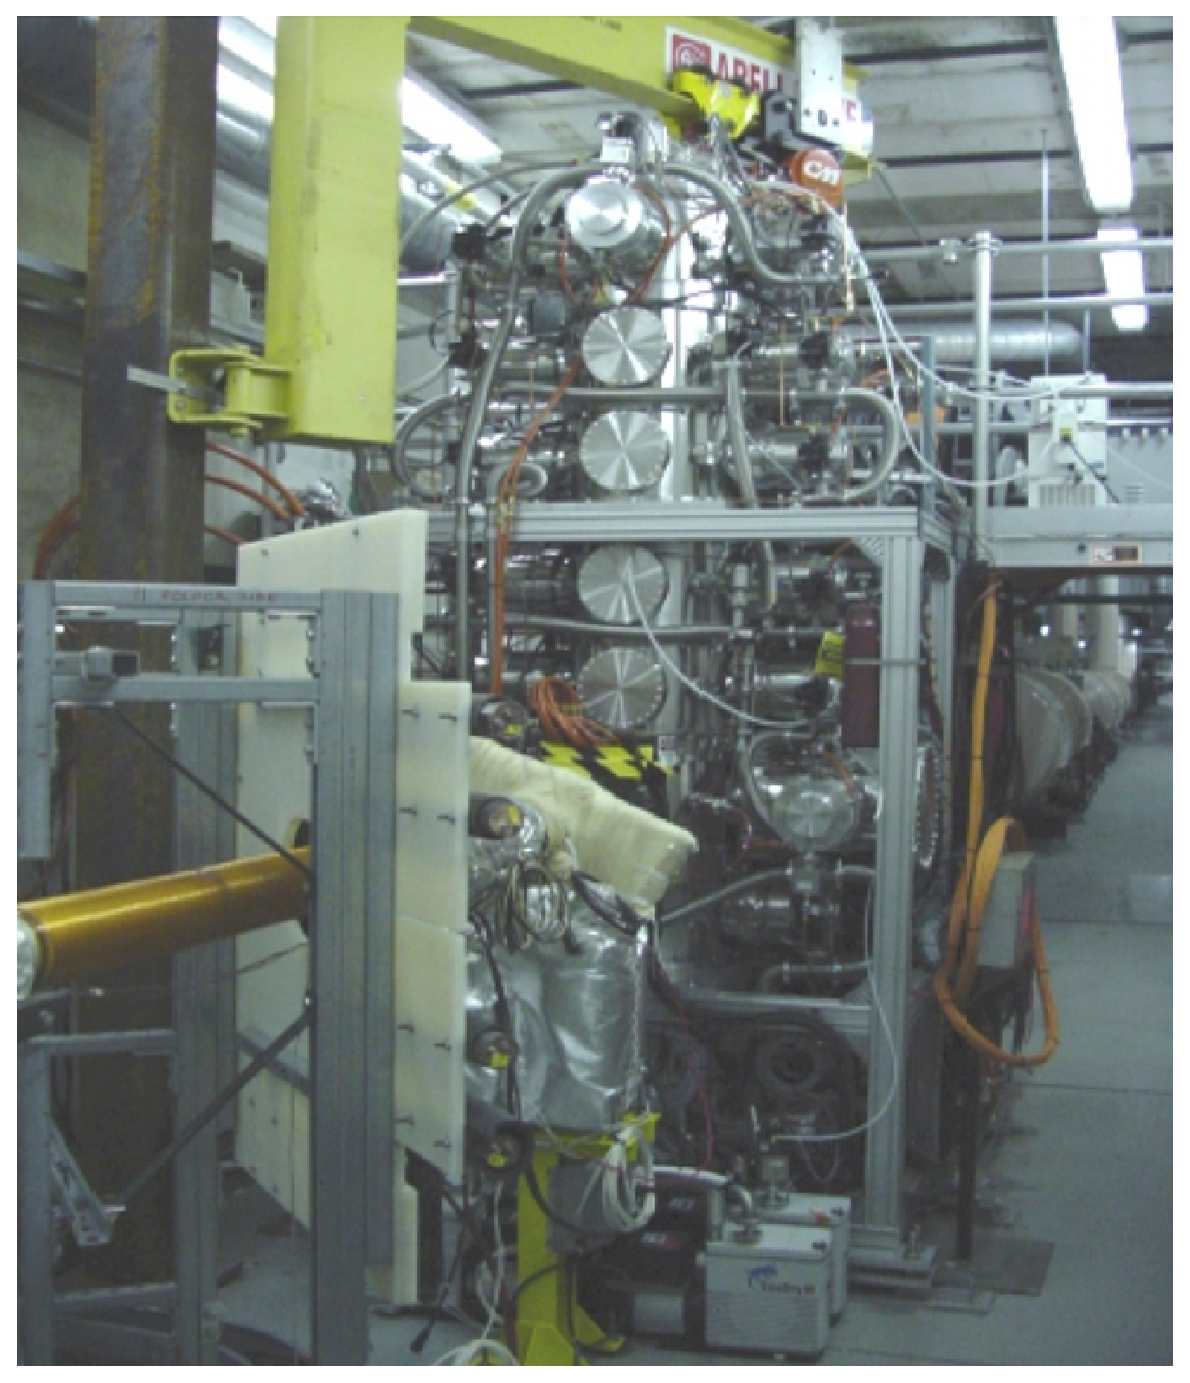
\includegraphics[height=20\unitlength]{graphics/jet}}
\rput[rt](49,30.5){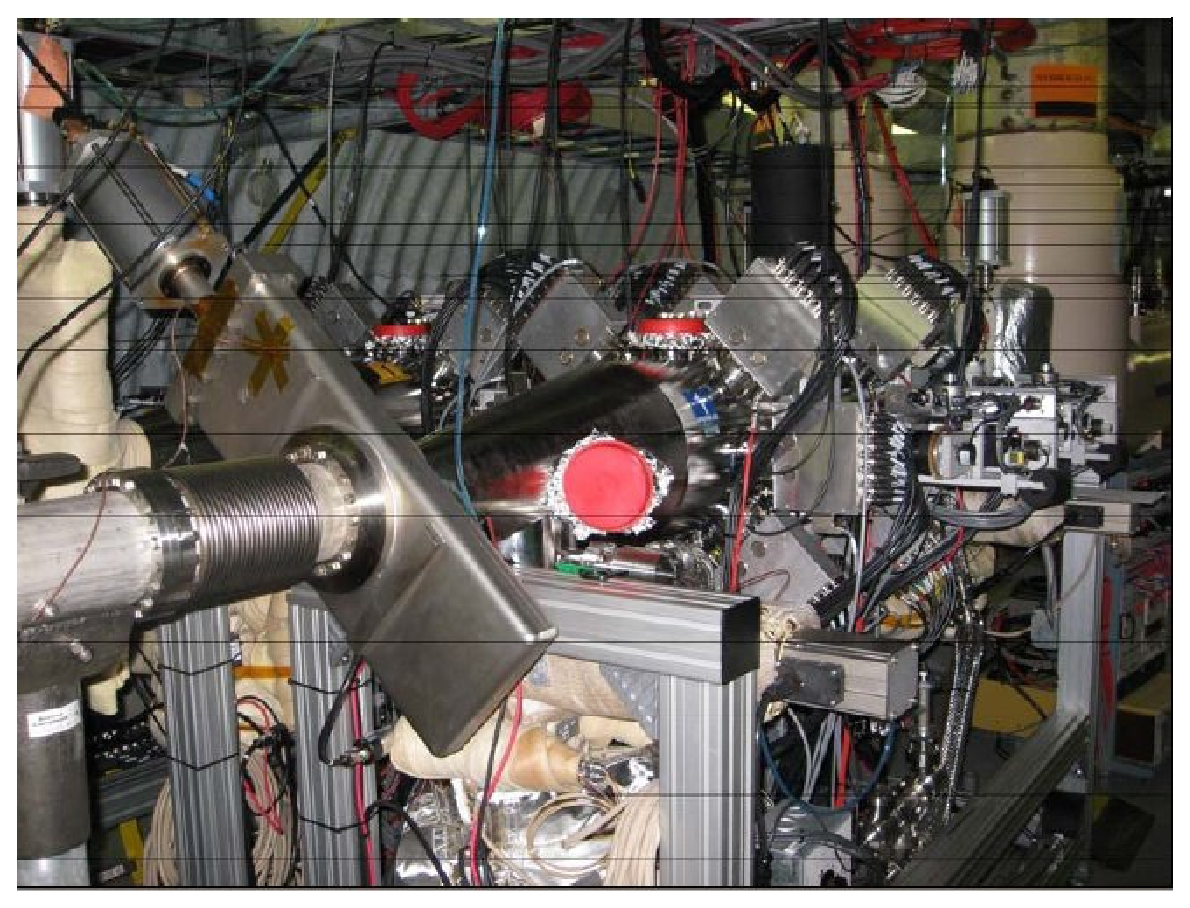
\includegraphics[height=20\unitlength]{graphics/pcarbon}}

\psline[linewidth=0.35, arrowscale=2, linecolor=green]{->}(12,26.5)(12,20.5)
\rput[lt](12.5,26.5){\textcolor{green}{\large \boldmath $H$}}

\psline[linewidth=0.35, arrowscale=2, linecolor=blue]{->}(3,16.5)(9,18)
\rput[lt](3,16){\textcolor{blue}{\large \boldmath $p$}}

\psline[linewidth=0.35, arrowscale=2, linecolor=blue]{->}(23,17.5)(29,19)
\rput[lt](23,17){\textcolor{blue}{\large \boldmath $p$}}

\psline[linewidth=0.1,linecolor=blueDark](21.5,-1)(21.5,30)

\rput[lt](0.5,10) {%
\begin{minipage}{20\unitlength}

\raggedright

\begin{list}{\labelitemi}{\setlength{\itemsep}{-3mm}
                          \setlength{\topsep}{0mm}}

   \item {\bf Hydrogen Jet Polarimeter}

   \small
   \begin{list}{\labelitemii}{\setlength{\itemsep}{0mm} \setlength{\topsep}{-2mm}}
      \item \textbf{Jet is polarized!}
      \item Continuous operation throughout the fill ($\sim 8-10$ hours)
      \item Provides \textbf{absolute average} polarization over the fill
      \item Lower statistical power
   \end{list}

\end{list}

\end{minipage}
}


\rput[lt](22,10) {%
\begin{minipage}{28\unitlength}

\raggedright

\begin{list}{\labelitemi}{\setlength{\itemsep}{-3mm}
                          \setlength{\topsep}{0mm}}

   \item {\bf p-Carbon Polarimeters\\(two in each ring)}

   \small
   \begin{list}{\labelitemii}{\setlength{\itemsep}{0mm} \setlength{\topsep}{-2mm}}
      \item About four $3$-minute measurements per fill
      \item Polarization decay in fill
      \item Beam polarization profiles\\[3mm]
      \item Higher statistical power
   \end{list}
\end{list}

\end{minipage}
}


%\rput{0}{\psgrid[gridlabels=0.7,subgriddiv=0, griddots=3](1,-1)(0,0)(\myPsPictureWidthLocal,\myPsPictureHeightLocal)}

}

\setlength{\unitlength}{10mm}
\psset{unit=\unitlength}
